
% 01-prologue/slides.tex, v. 1 (21/12/12)
% companion files to "Language and Computers"
% Dickinson, Brew, & Meurers (2013)

\documentclass{beamer}

\usepackage{graphicx}
\usepackage{tikz}

\usetikzlibrary{positioning,shapes,arrows,automata}
\def\dx{1cm} \def\dy{1.5cm}
\tikzstyle{state}=[draw,ellipse]

\newcommand{\newState}[4]{\node[state,#3](#1)[#4]{#2};}
\newcommand{\newTransition}[4]{\path[->] (#1) edge [#4] node {#3} (#2);} 
\usepackage{forest,adjustbox}
\useforestlibrary{linguistics}
\forestapplylibrarydefaults{linguistics}

\title{Introdução NLP e IR}
\author[]{Alexandre Rademaker\thanks{Olga Zamaraeva, University of Washington}}
\institute{FGV/EMAp}
\subtitle{Regular expressions and Finite State Automata}

\begin{document}
   
\begin{frame}
  \maketitle
\end{frame}

\section{Formal Language Theory}

\begin{frame}{So, we will talk about: Regular Expressions}
  \begin{itemize}
  \item sequence of characters that defines a (search) pattern
  \item $\backslash$([0-9]\{3\}$\backslash$)[0-9]\{3\}-[0-9]\{4\}
    \begin{itemize}
    \item matches phone numbers
    \end{itemize}
  \item You can play with regexes here:
    \begin{itemize}
    \item \url{https://regex101.com/}
    \end{itemize}
  \item RegEx as a tool:
  \item RegEx are equivalent to Finite State Automata 
  \item Fun fact: Kleene developed RegEx to describe the capabilities of early neural nets
  \end{itemize}
\end{frame}

\begin{frame}{Which are directly related to: \\ Finite State Automata}
colou?r

\vspace{0.5cm}

\{color; colour\}

\vspace{0.2cm}

\begin{center}
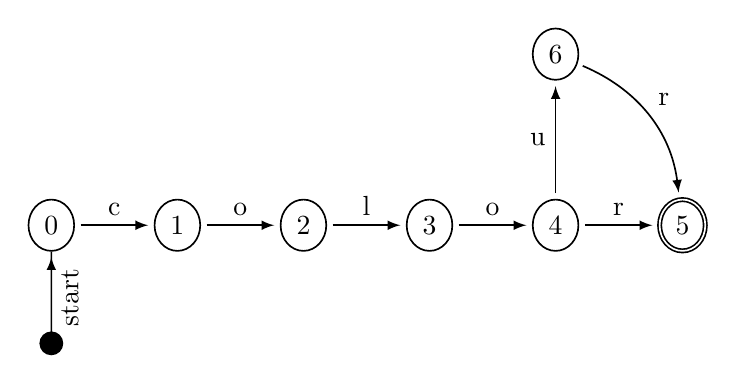
\begin{tikzpicture}[node distance=\dy and \dx,
  >=latex,shorten >=2pt,shorten <=2pt,auto,
  semithick  %semithick, thick, thin semithick
  ]
  \newState{q0}{$0$}{initial below,initial text={}}{}
  \newState{q1}{$1$}{right=of q0}{}
  \newState{q2}{$2$}{right=of q1}{}
  \newState{q3}{$3$}{right=of q2}{}
  \newState{q4}{$4$}{right=of q3}{}
  \newState{q6}{$6$}{above=of q4}{}
  \newState{q5}{$5$}{right=of q4}{accepting}
  \newTransition{q0}{q1}{c}{}
  \newTransition{q1}{q2}{o}{}
  \newTransition{q2}{q3}{l}{}
  \newTransition{q3}{q4}{o}{}
  \newTransition{q4}{q6}{u}{}
  \newTransition{q6}{q5}{r}{bend left}
  \newTransition{q4}{q5}{r}{}
  \draw[<-] (q0) -- node[midway,sloped,below,rotate=180] {start} ++(0,-\dy) [fill] circle (4pt);
  \end{tikzpicture}\end{center}
The two things are equivalent in that they ``generate'' the same set of strings
\end{frame}

\begin{frame}{Which describe: Regular Languages}

  ...which are part of the Chomsky Hierarchy:

  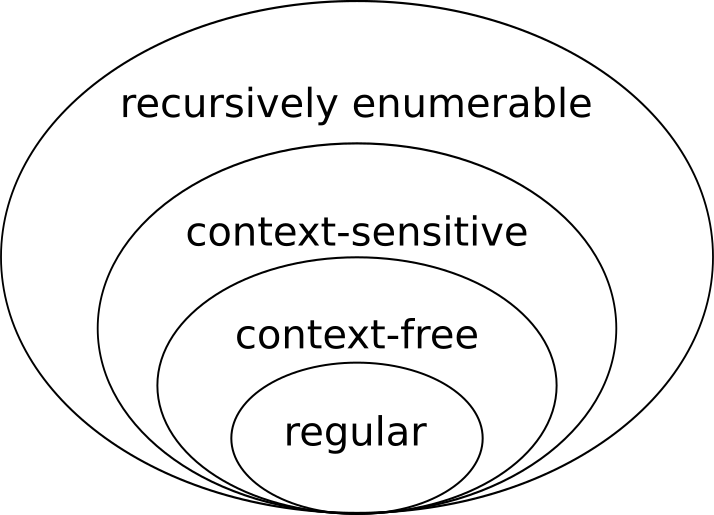
\includegraphics[width=.8\textwidth]{figures/chomsky-hier}

\tiny
picture from Wikipedia.
\end{frame}

%\begin{frame}
%\frametitle{Why is formal language complexity theory important?}
%\begin{itemize}
%\item  Formal language theory is connected to formal grammars
%\item Formal grammars represent structure on {\it computational level}
%\item It is a systematic study of patterns in languages
%\begin{itemize}
%	\item both artificial and natural
%\end{itemize}
%\item We would like to represent structure in language modeling
%\begin{itemize}
%\item always?..
%\end{itemize}
%\item Area of applicability:
%\begin{itemize}
%	\item Is it possible/necessary to formally describe a programming language?
%	\item ...a natural language?
%\end{itemize}
%\end{itemize}
%\end{frame}


\begin{frame}{What are formal languages?}

  Informally, a formal language is a set of strings (over some alphabet) and a set of rules.
  \vfill
  
  What about just enumerating all possible strings? Is this a language, formally?

\end{frame}

\begin{frame}{Formal languages}

$\sum=$\{a,b,c\} (alphabet)

$L=(a|b)c$ (regular language)
\vfill

\begin{itemize}
\item Formally, a \textit{grammar} (informally, set of rules)
  \textit{generate}s or \textit{accepts} (describes) a
  \textit{language} (set of strings defined over an alphabet).
\item One grammar has greater \textit{generative power} than the other
  if can define a language that the other cannot.
\item This is achieved by placing more or less constraints on how
  grammar rules can be written
\end{itemize}
\end{frame}

\begin{frame}{Formal languages: Definitions}

\begin{description}
\item[terminal] specific word
\item[non-terminal] generalization over a word, a class of words
\item[rewrite rule (production)] in what way can the symbols be grouped together?
\end{description}
\vfill

NP $\rightarrow$Det Nominal \\ 
NP $\rightarrow$ ProperNoun \\
Nominal $\rightarrow$ Noun$\vert$Nominal Noun \\
Det $\rightarrow$ the \\
Det $\rightarrow$ a \\
Noun $\rightarrow$ flight
\end{frame}

%\begin{frame}
%\frametitle{**Formal languages in a table}
%
%\small
%\begin{tabular}{clll}
%Type & Common Name & Rule Skeleton & Example \\
%\hline 
%0 & Turing equivalent & $\alpha \rightarrow \beta$ s.t. $\alpha \neq \epsilon$ & {\tiny HPSG, LFG}\\ 
%1 &  Context Sensitive & $\alpha A \beta \rightarrow \alpha \gamma \beta$ s.t. $\gamma \neq \epsilon$ & {\tiny phon. rules}\\
%- & Mildly Context Sensitive & & {\tiny CCG} \\
%2 & Context Free & $A \rightarrow \gamma $ & {\tiny CFG} \\
%3 & Regular (Right-Linear) & $A \rightarrow xB$ or $ A \rightarrow x $ & {\tiny FSA} \\
%3 & Regular (Left-Linear) & $A \rightarrow Bx$ or $ A \rightarrow x $ & {\tiny FSA} \\
%\hline
%\end{tabular}

%\vspace{0.5cm}
%
%A regular language {\bf cannot} express: $A \rightarrow xBx$ 
%
%\begin{itemize}
%\item {\it x} is a terminal
%\item $\alpha \beta \gamma$ are terminals or non-terminals, $\gamma$ can't be the empty string
%\item {\it A, B} are non-terminals
%\end{itemize}
%\end{frame}


\begin{frame}{The Turing Machine (1936; Alan Turing (1912-1954))}
\begin{small}
\begin{itemize}
\item A reading/writing head is moving along the tape, executing instructions (program).
\item \small ``Turing equivalent'' (or ``Turing complete''): no restrictions as to what you can write to the tape.
\item The most expressive language (can {\bf run any program}, including self)
\item Not actually a machine, it is a mental construct
\item In fact, engineers often try to avoid Turing-complete solutions (why?)
\end{itemize}
\end{small}
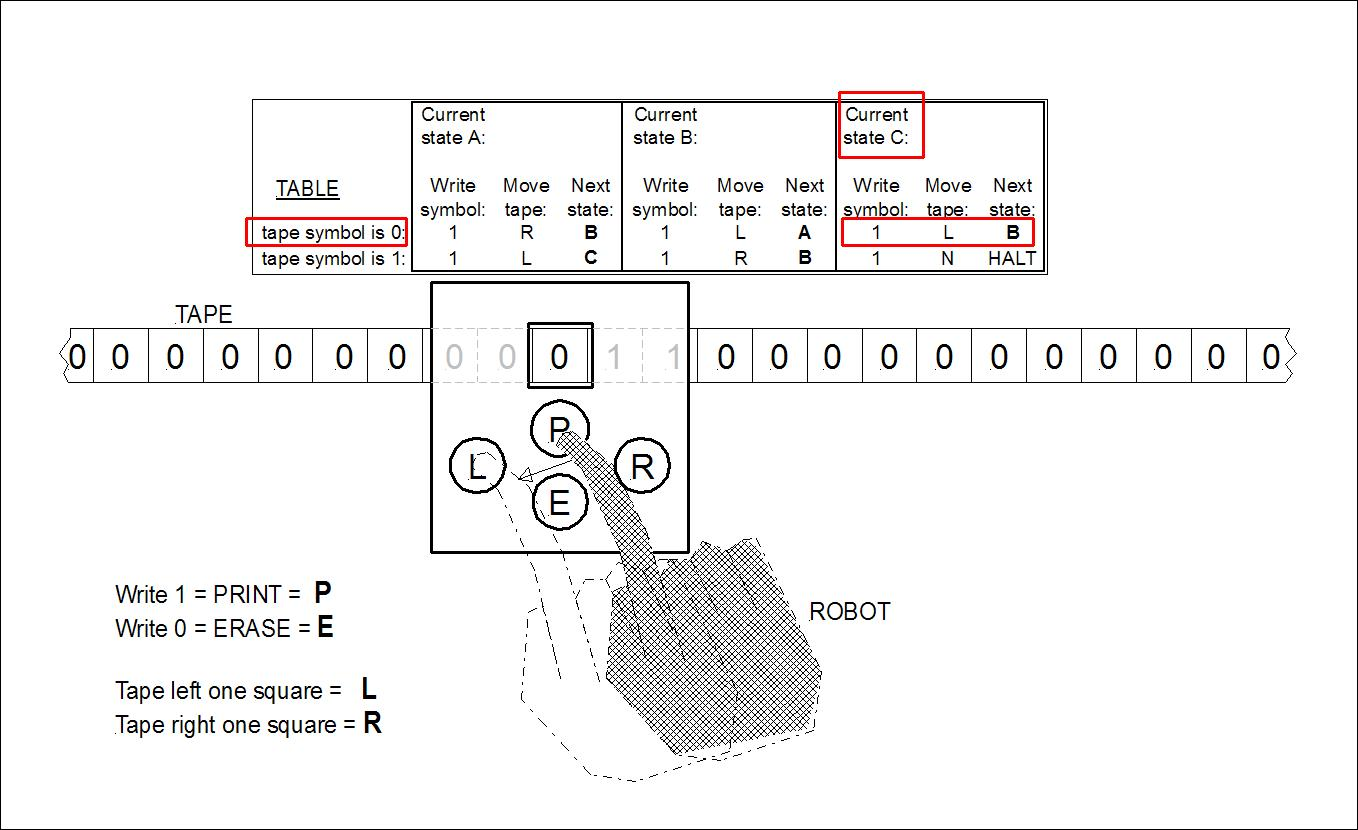
\includegraphics[height=0.3\textheight]{figures/turing}
\end{frame}

\begin{frame}{Why need subTuring languages?}
\begin{itemize}
\item Turing-complete languages are unbounded in power
\item Why bother with SubTuring languages, then?
\item ``Accidentally Turing-complete'': \url{http://beza1e1.tuxen.de/articles/accidentally_turing_complete.html}
\end{itemize}
\end{frame}

\begin{frame}{Natural language complexity}

{\it This is the malt that the rat that the cat that the dog worried killed ate.} -- Victor H. Yngve (1960)
\vfill

\begin{itemize}
\item {\it The Republicans who the senator who she voted for chastised were trying to cut all benefits for veterans. (J\&M, p. 529)}
\item What level of complexity occurs in natural language?
\item \textit{Models} of natural language differ in their \textit{power} with respect to levels of \textit{complexity}
\item What type of models do we end up using {\it in practice}?
\end{itemize}
\end{frame}


\begin{frame}{Natural language complexity}

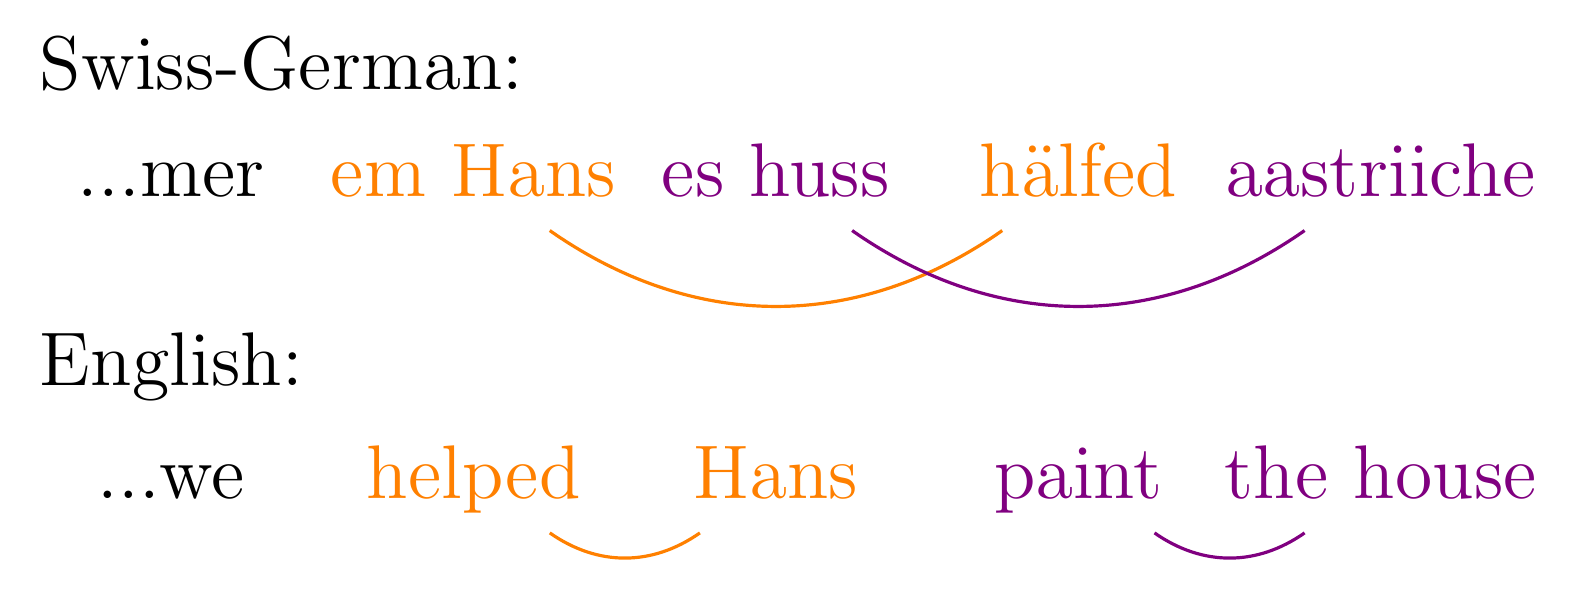
\includegraphics[width=.8\textwidth]{figures/swiss}

{\small \it ``It is generally agreed that natural languages ... are
  not regular, although most attempted proofs of this are widely known
  to be incorrect.''}

\small
Regular? 
\begin{itemize}
\item No, because recursion.
\item Recall the definition: a regular language is equivalent to a
  finite state automaton, while recursion requires potentially
  infinite stack
\end{itemize}
\end{frame}

\begin{frame}{Natural language complexity}

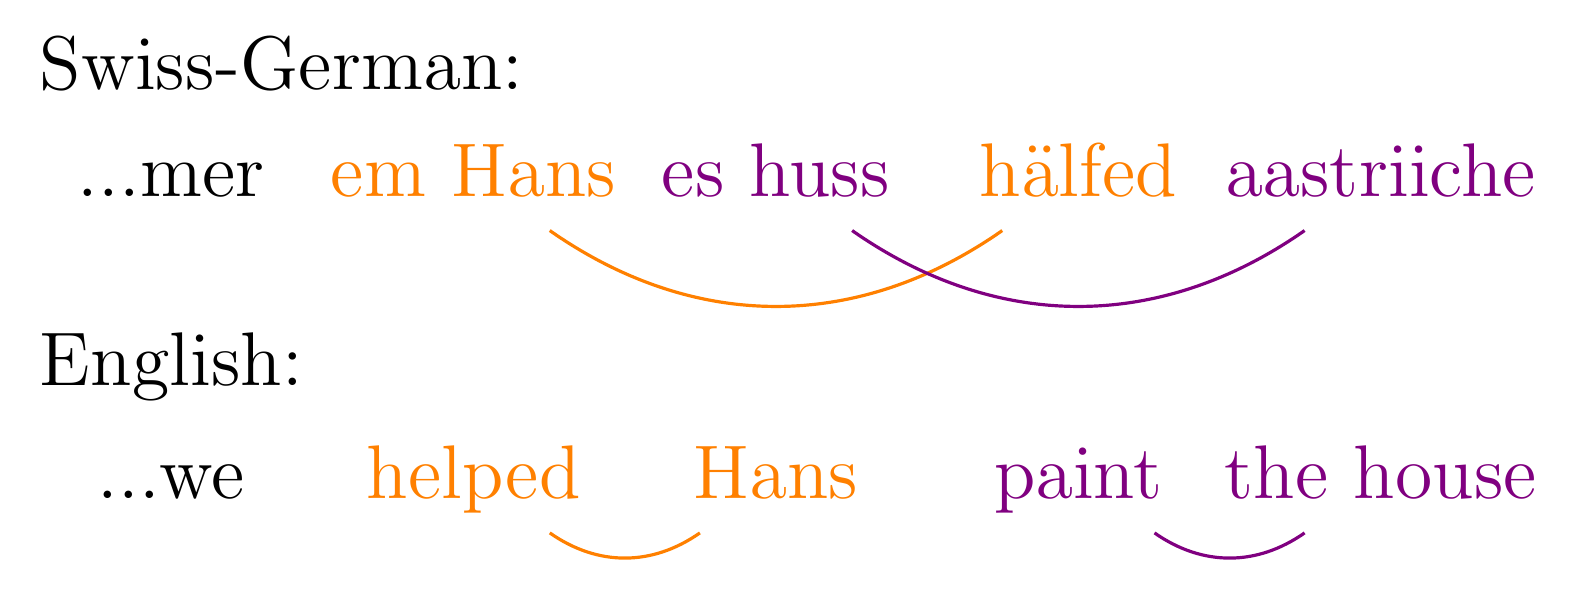
\includegraphics[width=\textwidth]{figures/swiss}

{\small \it ``It is generally agreed that natural languages ... are
  not regular, although most attempted proofs of this are widely known
  to be incorrect.''}

\small
\begin{itemize}
\item Context-free?
\begin{itemize}
\item Maybe, but maybe not, because Swiss German
\end{itemize}
\item Context-sensitive?
\begin{itemize}
\item $a^mb^nc^md^n...$
\item realistically, how big are $m$ and $n$?
\end{itemize}

\end{itemize}

%{\small NB: You can prove a language is not regular or not context-free, using {\it the Pumping Lemma.}}

\end{frame}

\begin{frame}{Why try to determine language complexity?}
  \begin{itemize}
  \item We know the expressive power of our models
  \item How adequate is model X for language Y?
    \begin{itemize}
    \item You want your program to react to certain input (language) in a certain way;
    \item If the model's capabilities wrt this input are {\bf limited}, better know that upfront
    \end{itemize}
  \item Are natural languages {\it really} context-sensitive?
    \begin{itemize}
    \item \ldots most programming languages are actually Turing-complete
    \item what might this mean for natural languages?
    \end{itemize}
  \end{itemize}
\end{frame}

\begin{frame}{Chomsky hierarchy and human language}

  What should the learner acquire?

  \vspace{0.2cm}
  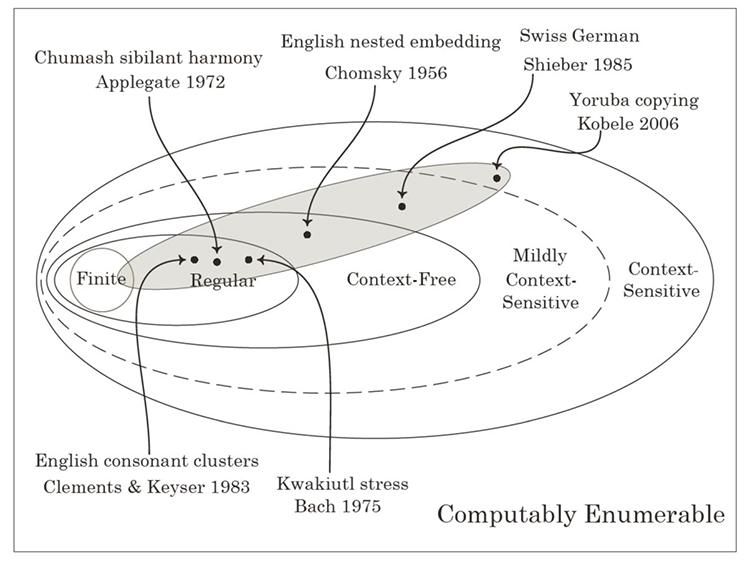
\includegraphics[width=.8\textwidth]{figures/fig03b}
  \tiny
  picture from Rawski \& Heinz. Language, vol. 95 no. 1, 2019, pp. e125-e135.
\end{frame}


\begin{frame}{Language complexity roadmap}
  \begin{itemize}
  \item We will start with regular languages by looking at regular
    expressions as search patterns and FSA for morphology 
  \item We can continue with context free grammars by looking at
    probabilistic context free parsing
  \item We can work with a Turing-complete\footnote{We won't really
      use the full power of the complexity.} language formalism (HPSG)
  \end{itemize}
\end{frame}

\section{Regular Languages}

\begin{frame}
\frametitle{Regular languages}
\begin{itemize}
\item At most one non-terminal on the LHS (left-hand side) and at most one terminal followed by one non-termial on the RHS.
\item $A \rightarrow xB$ or $ A \rightarrow x $ where x is a terminal and A,B are non-terminals
\end{itemize}

Language: {\bf a*bc*}

\hspace{3cm}
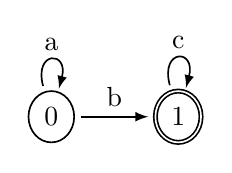
\begin{tikzpicture}[node distance=\dy and \dx,
  >=latex,shorten >=2pt,shorten <=2pt,auto,
  semithick  %semithick, thick, thin semithick
  ]
  \newState{S}{$0$}{}{}
  \newState{q1}{$1$}{right=of S}{accepting}
  \newTransition{S}{S}{a}{loop above}
  \newTransition{q1}{q1}{c}{loop above}
  \newTransition{S}{q1}{b}{}
  \end{tikzpicture}

  \begin{align*}
    S & \rightarrow aS \\
    S & \rightarrow bA \\
    A & \rightarrow \epsilon \\
    A & \rightarrow cA \\
  \end{align*}
\end{frame}

\begin{frame}{Three views of the same object}

  {\it Regular languages can be described by regular expressions or by finite state automata}

  \begin{itemize}
  \item Regular language: a set of strings
  \item Regular expressions compactly describes a regular language
  \item Finite State Automaton (FSA) accepts or generates all the strings from the language (and no other strings)
  \item In this sense, the FSA and the regular expression are ``equivalent'' to each other
  \end{itemize}
\end{frame}

\begin{frame}{Regular languages: Formal definition}

Required symbols:

\begin{itemize}
\item $\epsilon$ is the empty string
\item $\emptyset$ is the empty set
\item $\sum$ is an alphabet (e.g.\ $\sum = $\{a,b,c,d\})
\end{itemize}

The class of regular languages over $\sum$ is formally defined as: 

\begin{itemize}
\item $\emptyset$  is a regular language
\item $\forall$a $\in \sum \cup \epsilon$, \{a\} is a regular language  
\item If L1 and L2 are regular languages, then so are:
\begin{itemize}
\item L1 $\cdot$ L2 = \{xy $\vert$ x $\in$ L1, y $\in$ L2\} (concatenation)
\item L1 $\cup$ L2 (union or disjunction)
\item L1* (Kleene closure)
\end{itemize}
\end{itemize}
\end{frame}


\begin{frame}{The Pumping Lemma (intuition)}
  Why are languages of the form $a^nb^n$ not regular?

  aka: why it is not possible to model syntax with FSA?

  \url{https://en.wikipedia.org/wiki/Pumping_lemma_for_regular_languages}
\end{frame}

\section{Regular Expressions}

\newcommand{\A}{\texttt{\ensuremath{\,\hat{ }\,}}}

\begin{frame}{Regular expressions: Tools that use them}
  \begin{itemize}
  \item A variety of unix tools (grep, sed, tr, awk \ldots), editors
    (emacs, jEdit, \ldots), and programming languages (perl, python,
    Java, \ldots) incorporate regular expressions.
        
  \item Implementations are fairly efficient, but regex are still slow
    as far as computers go
    
  \item The various tools and languages differ w.r.t. the exact syntax
    of the regular expressions they allow but all are similar.
  \end{itemize}
\end{frame}


\begin{frame}[allowframebreaks]{The syntax of regular expressions}

  Regular expressions consist of
  
  \begin{itemize}
  \item strings of literal characters: \texttt{c}, \texttt{A100},
    \texttt{natural language}, \texttt{30 years!}
  \item disjunction:
    \begin{itemize}
    \item ordinary disjunction: \texttt{famil(y|ies)}
    \item character classes: \texttt{[Tt]he}, \texttt{bec[oa]me}
    \item ranges: \texttt{[A-Z]} (any capital letter)
    \end{itemize}
    
  \item negation: 
    \mbox{\begin{tabular}[t]{@{}l@{}}
            \texttt{[{\A}a]} (any symbol but \texttt{a})\\
            \texttt{[{\A}A-Z0-9]} (not an uppercase letter or number)
          \end{tabular}}
  \end{itemize}

  \framebreak

  \begin{itemize}
  \item counters
    \begin{itemize}
    \item optionality: \texttt{?}\\
      \texttt{colou?r}
    \item any number of occurrences: \texttt{*} (Kleene star)\\
      \texttt{[0-9]* years}
    \item at least one  occurrence: \texttt{+}\\
      \texttt{[0-9]+ dollars}
    \end{itemize}
  \item wildcard for any character: .\\
    \texttt{beg.n} for any character in between \texttt{beg} and \texttt{n} 
  \end{itemize}

  \framebreak

  \begin{itemize}
  \item Escaped characters: to specify a character with a special
    meaning (\texttt{*}, \texttt{+}, \texttt{?}, \texttt{(}, \texttt{)},
    \texttt{|}, \texttt{[}, \texttt{]}) it is preceded by a backslash
    (\texttt{$\backslash$})
    
    e.g., a period is expressed as \texttt{$\backslash$.}

  \item Operator precedence, from highest to lowest:
    \begin{itemize}
    \item[] parentheses \texttt{()}
    \item[] counters \texttt{* + ?}
    \item[] character sequences
    \item[] disjunction \texttt{|}
    \end{itemize}
  \end{itemize}
\end{frame}


\begin{frame}{Regular expressions in python programming language}
  \begin{itemize}
  \item \url{https://docs.python.org/3/library/re.html} 
    
  \item (do study the above docs whenever you have a problem, rather
    than quickly looking at them and then trying to guess why you have a
    problem)
  \item Your best friend: \url{https://regex101.com/}
  \end{itemize}
\end{frame}


\begin{frame}[t]{RegEx example: Single character}
  \begin{itemize}
  \item Alphabet: $\sum$ = \{a\}
  \item Language (set of strings): L = \{a\}
  \item Regular expression: a
  \item FSA:
  \end{itemize}

  \pause

  \begin{center}
    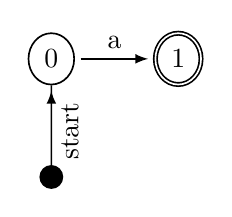
\begin{tikzpicture}[node distance=\dy and \dx,
      >=latex,shorten >=2pt,shorten <=2pt,auto,
      semithick  %semithick, thick, thin semithick
      ]
      \newState{S}{$0$}{initial below,initial text={}}{}
      \newState{q1}{$1$}{right=of S}{accepting}
      \newTransition{S}{q1}{a}{}
      \draw[<-] (S) -- node[midway,sloped,below,rotate=180] {start} ++(0,-\dy) [fill] circle (4pt);
    \end{tikzpicture}\end{center}
\end{frame}

\begin{frame}[t]{RegEx example: Disjunction/Union}
  \begin{itemize}
  \item Alphabet: $\sum$ = \{a,b\}
  \item Language (set of strings): L = \{a,b\}
  \item Regular expression: a$\vert$b
  \item FSA:
  \end{itemize}

  \pause 
  
  \begin{center}
    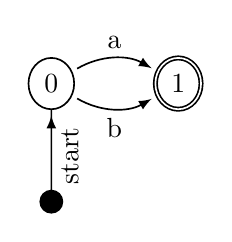
\begin{tikzpicture}[node distance=\dy and \dx,
      >=latex,shorten >=2pt,shorten <=2pt,auto,
      semithick  %semithick, thick, thin semithick
      ]
      \newState{S}{$0$}{initial below,initial text={}}{}
      \newState{q1}{$1$}{right=of S}{accepting}
      \newTransition{S}{q1}{a}{bend left}
      \newTransition{S}{q1}{b}{below,bend right}
      \draw[<-] (S) -- node[midway,sloped,below,rotate=180] {start} ++(0,-\dy) [fill] circle (4pt);
    \end{tikzpicture}\end{center}
\end{frame}

\begin{frame}[t]{RegEx example: Concatenation}
  \begin{itemize}
  \item Alphabet: $\sum$ = \{a,b,c,d\}
  \item Language (set of strings): L1 = \{a,b\}, L2 = \{c,d\}
  \item Regular expression: (a$\vert$b)$\cdot$(c$\vert$d)
  \item FSA:
  \end{itemize}

  \pause
    
  \begin{center}
    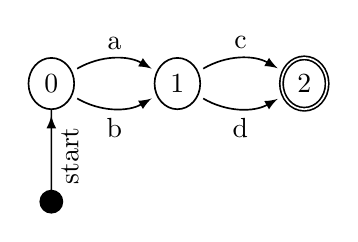
\begin{tikzpicture}[node distance=\dy and \dx,
      >=latex,shorten >=2pt,shorten <=2pt,auto,
      semithick  %semithick, thick, thin semithick
      ]
      \newState{S}{$0$}{initial below,initial text={}}{}
      \newState{q1}{$1$}{right=of S}{}
      \newState{q2}{$2$}{right=of q1}{accepting}
      
      \newTransition{S}{q1}{a}{bend left}
      \newTransition{S}{q1}{b}{below,bend right}
      \newTransition{q1}{q2}{c}{bend left}
      \newTransition{q1}{q2}{d}{below,bend right}
      \draw[<-] (S) -- node[midway,sloped,below,rotate=180] {start} ++(0,-\dy) [fill] circle (4pt);
    \end{tikzpicture}
  \end{center}
  
   what about: (ab)$\vert$(cd)?
\end{frame}


\begin{frame}[t]{RegEx example: Kleene closure}
  \begin{itemize}
  \item Alphabet: $\sum$ = \{a,b\}
  \item Language (set of strings): L1 = \{$\epsilon$,a,b,aa,bb,ab,ba,bb...\}
  \item Regular expression: (a$\vert$b)*
  \item FSA:
  \end{itemize}

  \pause 

  \begin{center}
    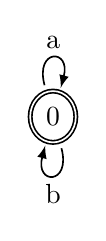
\begin{tikzpicture}[node distance=\dy and \dx,
      >=latex,shorten >=2pt,shorten <=2pt,auto,
      semithick  %semithick, thick, thin semithick
      ]
      \newState{S}{$0$}{}{accepting} 
      \newTransition{S}{S}{a}{loop above}
      \newTransition{S}{S}{b}{loop below}
  \end{tikzpicture}\end{center}
\end{frame}

\begin{frame}[t]
\frametitle{FSA as transition table}
\begin{center}
  \begin{tabular}{|l|c|c|c|}
    \hline
    State & a & b & c \\
    \hline
    $>$0 & 1 & 3 & - \\
    \hline 
    1 & 1 & 2 & - \\
    \hline
    2: & - & 3 & 3 \\
    \hline
    3: & - & - & - \\
    \hline
  \end{tabular}
\end{center}
\end{frame}


\section{FSA}

\begin{frame}[t]{FSA as transition table}
  \begin{center}
    \begin{tabular}{|l|c|c|c|}
      \hline
State & a & b & c \\
      \hline
      $>$0 & 1 & 3 & - \\
      \hline 
      1 & 1 & 2 & - \\
      \hline
      2: & - & 3 & 3 \\
      \hline
      3: & - & - & - \\
      \hline
    \end{tabular}
  \end{center}
  
  \begin{center}
    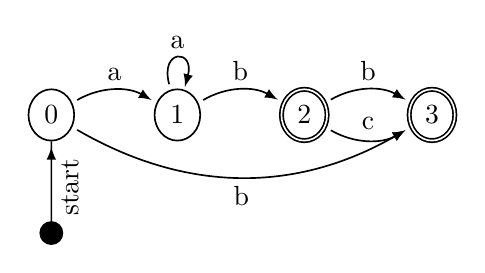
\begin{tikzpicture}[node distance=\dy and \dx,
      >=latex,shorten >=2pt,shorten <=2pt,auto,
      semithick  %semithick, thick, thin semithick
      ]
      \newState{S}{$0$}{initial below,initial text={}}{}
      \newState{q1}{$1$}{right=of S}{}
      \newState{q2}{$2$}{right=of q1}{accepting}
      \newState{q3}{$3$}{right=of q2}{accepting}
      
      \newTransition{S}{q1}{a}{bend left}
      \newTransition{q1}{q2}{b}{bend left}
      \newTransition{q1}{q1}{a}{loop above}
      \newTransition{q2}{q3}{b}{bend left}
      \newTransition{q2}{q3}{c}{bend right}
      \newTransition{S}{q3}{b}{below, bend right}
      \draw[<-] (S) -- node[midway,sloped,below,rotate=180] {start} ++(0,-\dy) [fill] circle (4pt);
    \end{tikzpicture}
  \end{center}
\end{frame}

\begin{frame}{DFSA and NFSA}
  \begin{itemize}\small
  \item \textbf{Deterministic Finite State Automaton (DFSA, DFA)}
    \begin{itemize}
    \item Does not have ``free'' ($\epsilon$, empty string) transitions
    \item (Meaning: State changes only after reading an input)
    \item Given an input sequence, you can predict uniquely the next state
    \end{itemize}
  \end{itemize}
  \begin{center}
    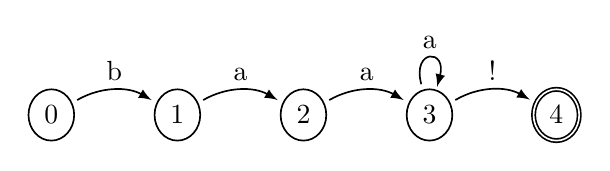
\begin{tikzpicture}[node distance=\dy and \dx,
      >=latex,shorten >=2pt,shorten <=2pt,auto,
      semithick  %semithick, thick, thin semithick
      ]
      \newState{S}{$0$}{}{}
      \newState{q1}{$1$}{right=of S}{}
      \newState{q2}{$2$}{right=of q1}{}
      \newState{q3}{$3$}{right=of q2}{}
      \newState{q4}{$4$}{right=of q3}{accepting}
      \newTransition{S}{q1}{b}{bend left}
      \newTransition{q1}{q2}{a}{bend left}
      \newTransition{q2}{q3}{a}{bend left}
      \newTransition{q3}{q3}{a}{loop above}
      \newTransition{q3}{q4}{!}{bend left}
    \end{tikzpicture}
  \end{center}
  \small
  \begin{itemize}
  \item \textbf{Nondeterministic Finite State Automaton (NFSA, NFA)}
    \begin{itemize}
    \item Can have ``free'' ($\epsilon$, empty string) transitions
    \item Given an input sequence, you can't always predict the next state
    \item Can be convenient, e.g.\ to convert regex to a FSA
    \end{itemize}
  \end{itemize}
  \begin{center}
    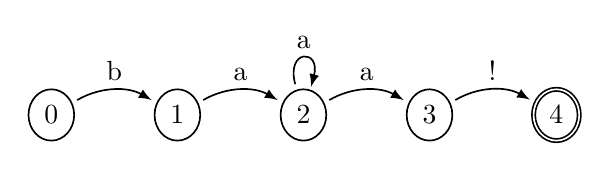
\begin{tikzpicture}[node distance=\dy and \dx,
      >=latex,shorten >=2pt,shorten <=2pt,auto,
      semithick  %semithick, thick, thin semithick
      ]
      \newState{S}{$0$}{}{}
      \newState{q1}{$1$}{right=of S}{}
      \newState{q2}{$2$}{right=of q1}{}
      \newState{q3}{$3$}{right=of q2}{}
      \newState{q4}{$4$}{right=of q3}{accepting}
      \newTransition{S}{q1}{b}{bend left}
      \newTransition{q1}{q2}{a}{bend left}
      \newTransition{q2}{q3}{a}{bend left}
      \newTransition{q2}{q2}{a}{loop above}
      \newTransition{q3}{q4}{!}{bend left}
    \end{tikzpicture}
  \end{center}
\end{frame}


\begin{frame}{Converting FSA to RegEx}

  E.g.\ The State Removal method
  \begin{itemize}
  \item If transitions out of Start state:
    \begin{itemize}
    \item Add a new Start state
    \item Old Start state no longer start
    \item Add an $\epsilon$ transition from new Start to old
    \end{itemize}
  \item If more that one Accepting state or transitions out of Accepting state:
    \begin{itemize}
    \item Add a new Accepting State
    \item Add $\epsilon$ transitions from old Accepting states to new
    \item Old Accepting states no longer accept
    \end{itemize}
  \item Now, remove intermediate states one by one, combining simple
    inputs on the edges into more complex inputs.  (Choose the
    simplest nodes to remove)
  \end{itemize}

  This algorithm is easy to visualize but harder to apply
  systematically. Look up e.g.\ {\it transition closure method} if you
  want systematic.
\end{frame}


\begin{frame}[allowframebreaks]{The State Removal Method}
  \small
  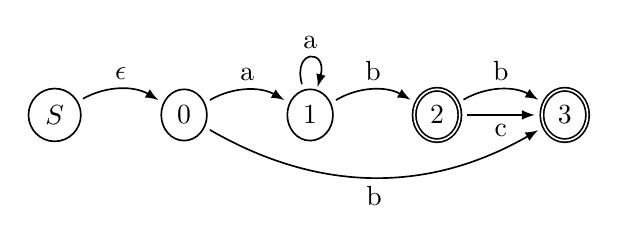
\begin{tikzpicture}[node distance=\dy and \dx,
    >=latex,shorten >=2pt,shorten <=2pt,auto,
    semithick  %semithick, thick, thin semithick
    ]
    \newState{SS}{$S$}{}{}
    \newState{S}{$0$}{right=of SS}{}
    \newState{q1}{$1$}{right=of S}{}
    \newState{q2}{$2$}{right=of q1}{accepting}
    \newState{q3}{$3$}{right=of q2}{accepting}
    \newTransition{SS}{S}{$\epsilon$}{bend left}
    \newTransition{S}{q1}{a}{bend left}
    \newTransition{q1}{q2}{b}{bend left}
    \newTransition{q1}{q1}{a}{loop above}
    \newTransition{q2}{q3}{b}{bend left}
    \newTransition{q2}{q3}{c}{below}
    \newTransition{S}{q3}{b}{below, bend right}
  \end{tikzpicture}
  
  \vspace{0.5cm}
  
  Getting rid of multiple accepting states:
  
  \vspace{1.5cm}
  
  Getting rid of State 1:

  \framebreak
  
  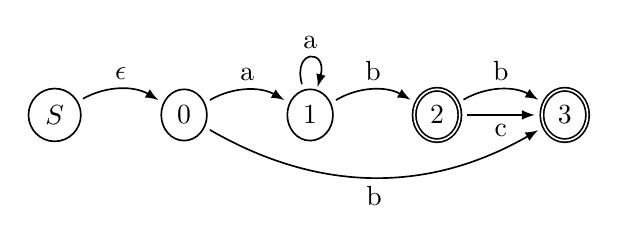
\begin{tikzpicture}[node distance=\dy and \dx,
    >=latex,shorten >=2pt,shorten <=2pt,auto,
    semithick  %semithick, thick, thin semithick
    ]
    \newState{SS}{$S$}{}{}
    \newState{S}{$0$}{right=of SS}{}
    \newState{q1}{$1$}{right=of S}{}
    \newState{q2}{$2$}{right=of q1}{accepting}
    \newState{q3}{$3$}{right=of q2}{accepting}
    \newTransition{SS}{S}{$\epsilon$}{bend left}
    \newTransition{S}{q1}{a}{bend left}
    \newTransition{q1}{q2}{b}{bend left}
    \newTransition{q1}{q1}{a}{loop above}
    \newTransition{q2}{q3}{b}{bend left}
    \newTransition{q2}{q3}{c}{below}
    \newTransition{S}{q3}{b}{below, bend right}
  \end{tikzpicture}
 
  Getting rid of multiple accepting states:
  
  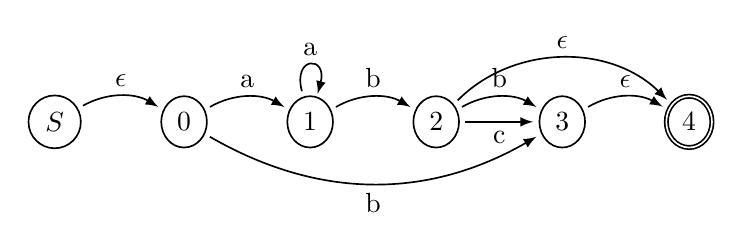
\begin{tikzpicture}[node distance=\dy and \dx,
    >=latex,shorten >=2pt,shorten <=2pt,auto,
    semithick  %semithick, thick, thin semithick
    ]
    \newState{SS}{$S$}{}{}
    \newState{S}{$0$}{right=of SS}{}
    \newState{q1}{$1$}{right=of S}{}
    \newState{q2}{$2$}{right=of q1}{}
    \newState{q3}{$3$}{right=of q2}{}
    \newState{q4}{$4$}{right=of q3}{accepting}
    \newTransition{SS}{S}{$\epsilon$}{bend left}
    \newTransition{S}{q1}{a}{bend left}
    \newTransition{q1}{q2}{b}{bend left}
    \newTransition{q1}{q1}{a}{loop above}
    \newTransition{q2}{q3}{b}{bend left}
    \newTransition{q2}{q3}{c}{below}
    \newTransition{S}{q3}{b}{below, bend right}
    \newTransition{q2}{q4}{$\epsilon$}{above, bend left=45}
    \newTransition{q3}{q4}{$\epsilon$}{bend left}
  \end{tikzpicture}
  
  Getting rid of State 1:
   
  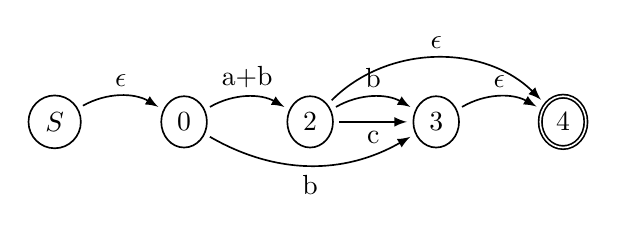
\begin{tikzpicture}[node distance=\dy and \dx,
    >=latex,shorten >=2pt,shorten <=2pt,auto,
    semithick  %semithick, thick, thin semithick
    ]
    \newState{SS}{$S$}{}{}
    \newState{S}{$0$}{right=of SS}{}
    \newState{q2}{$2$}{right=of S}{}
    \newState{q3}{$3$}{right=of q2}{}
    \newState{q4}{$4$}{right=of q3}{accepting}
    \newTransition{SS}{S}{$\epsilon$}{bend left}       
    \newTransition{S}{q2}{a+b}{bend left}
    \newTransition{q2}{q3}{b}{bend left}
    \newTransition{q2}{q3}{c}{below}
    \newTransition{S}{q3}{b}{below, bend right}
    \newTransition{q2}{q4}{$\epsilon$}{above, bend left=45}
    \newTransition{q3}{q4}{$\epsilon$}{bend left}
  \end{tikzpicture}

  \framebreak
  
  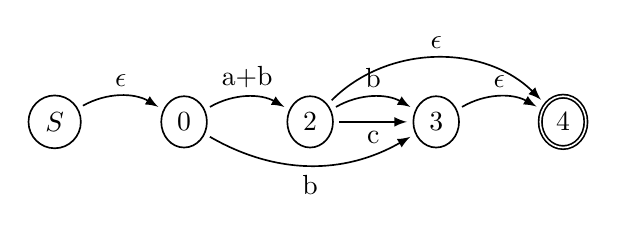
\begin{tikzpicture}[node distance=\dy and \dx,
    >=latex,shorten >=2pt,shorten <=2pt,auto,
    semithick  %semithick, thick, thin semithick
    ]
    \newState{SS}{$S$}{}{}
    \newState{S}{$0$}{right=of SS}{}
    \newState{q2}{$2$}{right=of S}{}
    \newState{q3}{$3$}{right=of q2}{}
    \newState{q4}{$4$}{right=of q3}{accepting}
    \newTransition{SS}{S}{$\epsilon$}{bend left}       
    \newTransition{S}{q2}{a+b}{bend left}
    \newTransition{q2}{q3}{b}{bend left}
    \newTransition{q2}{q3}{c}{below}
    \newTransition{S}{q3}{b}{below, bend right}
    \newTransition{q2}{q4}{$\epsilon$}{above, bend left=45}
    \newTransition{q3}{q4}{$\epsilon$}{bend left}
  \end{tikzpicture}

  \vspace{0.1cm}
  
  Getting rid of State 3:

  \vspace{1.5cm}
  
  Getting rid of State 2:

  \framebreak

  Getting rid of State 3:
  
  \begin{tikzpicture}[node distance=\dy and \dx,
    >=latex,shorten >=2pt,shorten <=2pt,auto,
    semithick  %semithick, thick, thin semithick
    ]
    \newState{SS}{$S$}{}{}
    \newState{S}{$0$}{right=of SS}{}
    \newState{q2}{$2$}{right=of S}{}
    \newState{q4}{$4$}{right=of q3}{accepting}
    \newTransition{SS}{S}{$\epsilon$}{bend left}       
    \newTransition{S}{q2}{a+b}{bend left}
    \newTransition{q2}{q4}{(b$\vert$c)?}{bend left}
    \newTransition{S}{q4}{b}{below, bend right}
  \end{tikzpicture}
  
  Getting rid of State 2:
  
  \begin{tikzpicture}[node distance=\dy and \dx,
    >=latex,shorten >=2pt,shorten <=2pt,auto,
    semithick  %semithick, thick, thin semithick
    ]
    \newState{SS}{$S$}{}{}
    \newState{S}{$0$}{right=of SS}{}
    \newState{q4}{$4$}{right=of q3}{accepting}
    \newTransition{SS}{S}{$\epsilon$}{bend left}  
    \newTransition{S}{q4}{a+b(b$\vert$c)?}{bend left}     
    \newTransition{S}{q4}{b}{below, bend right}
  \end{tikzpicture}

  The final picture yields the regular expression:
  \[
    (a+b(b \vert c)?) \vert b
  \]
\end{frame}


\begin{frame}{Converting regex to FSA (Thompson's construction)}
  \begin{itemize}
  \item Basically reversing the process above (with a bit more
    $\epsilon$ involved, if you want to follow the general case).
  
  \item (Why so many epsilon-transitions?  Thompson construction
    assumes strictly 1 entry and 1 exit point for each state)

  \item you are operating not just on nodes in a graph, but on
    separate {\it automata}, so you need to preserve their start and
    accepting states
\end{itemize}
\end{frame}


\begin{frame}[t]{Converting regex to FSA: regex to NFA}

a*(b$\vert$c)

\pause

a* (NFA, Kleene star of a):

\begin{center}
  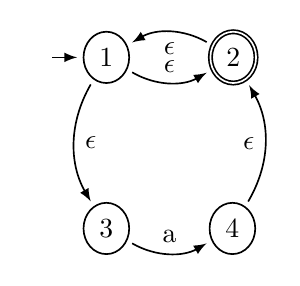
\begin{tikzpicture}[node distance=\dy and \dx,
    >=latex,shorten >=2pt,shorten <=2pt,auto,
    semithick  %semithick, thick, thin semithick
    ]
    \newState{q1}{$1$}{initial left,initial text={}}{}
    \newState{q2}{$2$}{right=of q1}{accepting}
    \newState{q3}{$3$}{below=of q1}{}
    \newState{q4}{$4$}{right=of q3}{}
    \newTransition{q1}{q2}{$\epsilon$}{bend right}
    \newTransition{q2}{q1}{$\epsilon$}{below, bend right}
    \newTransition{q1}{q3}{$\epsilon$}{bend right}
    \newTransition{q3}{q4}{a}{bend right}
    \newTransition{q4}{q2}{$\epsilon$}{bend right}
  \end{tikzpicture}
\end{center}
\end{frame}


\begin{frame}[t]{Converting regex to FSA: regex to NFA}

a*(b$\vert$c)

b$\vert$c (NFA, disjunction of b and c):
\begin{center}
  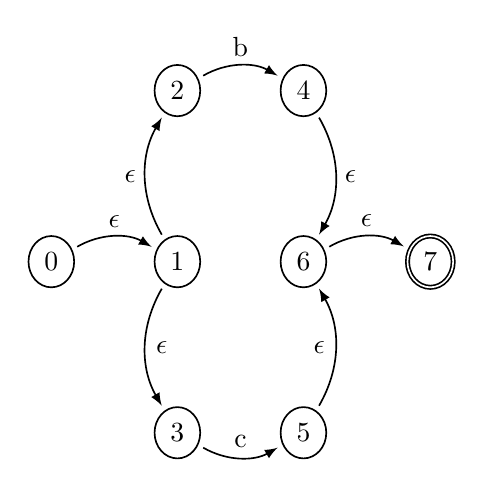
\begin{tikzpicture}[node distance=\dy and \dx,
    >=latex,shorten >=2pt,shorten <=2pt,auto,
    semithick  %semithick, thick, thin semithick
    ]
    \newState{S}{$0$}{}{}
    \newState{q1}{$1$}{right=of S}{}
    \newState{q2}{$2$}{above=of q1}{}
    \newState{q3}{$3$}{below=of q1}{}
    \newState{q4}{$4$}{right=of q2}{}
    \newState{q5}{$5$}{right=of q3}{}
    \newState{q6}{$6$}{right=of q1}{}
    \newState{q7}{$7$}{right=of q6}{accepting}
    \newTransition{S}{q1}{$\epsilon$}{bend left}
    \newTransition{q1}{q2}{$\epsilon$}{bend left}
    \newTransition{q1}{q3}{$\epsilon$}{bend right}
    \newTransition{q2}{q4}{b}{bend left}
    \newTransition{q3}{q5}{c}{bend right}
    \newTransition{q5}{q6}{$\epsilon$}{bend right}
    \newTransition{q4}{q6}{$\epsilon$}{bend left}
    \newTransition{q6}{q7}{$\epsilon$}{bend left}
  \end{tikzpicture}
\end{center}
\end{frame}



\begin{frame}[t]{Converting regex to FSA: regex to NFA}

a*(b$\vert$c)

a*(b$\vert$c) (NFA, concatenation of a* and b$\vert$c):

\vspace{0.5cm}

{\footnotesize Note: we can get from 0 to 4 by \textit{a}; from 4 to 4
  by \textit{a}; from 4 to 10 by \textit{b}; from 4 to 11 by
  \textit{c}. From 10 and 11, we can just halt.}

\begin{center}
  \resizebox{\textwidth}{0.5\textheight}{%
    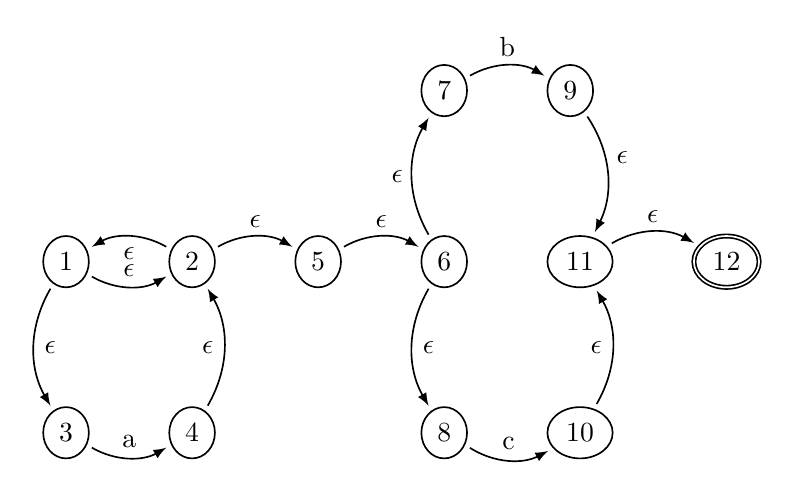
\begin{tikzpicture}[node distance=\dy and \dx,
      >=latex,shorten >=2pt,shorten <=2pt,auto,
      semithick  %semithick, thick, thin semithick
      ]
      % \newState{S1}{$0$}{}{}
      \newState{q1}{$1$}{}{}
      \newState{q2}{$2$}{right=of q1}{}
      \newState{q3}{$3$}{below=of q1}{}
      \newState{q4}{$4$}{right=of q3}{}
      % \newState{q5}{$5$}{right=of q2}{}
      % \newTransition{S}{q1}{$\epsilon$}{bend left}
      \newTransition{q1}{q2}{$\epsilon$}{bend right}
      \newTransition{q2}{q1}{$\epsilon$}{below, bend right}
      \newTransition{q1}{q3}{$\epsilon$}{bend right}
      \newTransition{q3}{q4}{a}{bend right}
      \newTransition{q4}{q2}{$\epsilon$}{bend right}
      % \newTransition{q2}{q5}{$\epsilon$}{bend left}
      \newState{S2}{$5$}{right=of q2}{}
      \newState{q6}{$6$}{right=of S2}{}
      \newState{q7}{$7$}{above=of q6}{}
      \newState{q8}{$8$}{below=of q6}{}
      \newState{q9}{$9$}{right=of q7}{}
      \newState{q10}{$10$}{right=of q8}{}
      \newState{q11}{$11$}{right=of q6}{}
      \newState{q12}{$12$}{right=of q11}{accepting}
      \newTransition{q2}{S2}{$\epsilon$}{bend left}
      \newTransition{S2}{q6}{$\epsilon$}{bend left}
      \newTransition{q6}{q7}{$\epsilon$}{bend left}
      \newTransition{q6}{q8}{$\epsilon$}{bend right}
      \newTransition{q7}{q9}{b}{bend left}
      \newTransition{q8}{q10}{c}{bend right}
      \newTransition{q9}{q11}{$\epsilon$}{bend left}
      \newTransition{q10}{q11}{$\epsilon$}{bend right}
      \newTransition{q11}{q12}{$\epsilon$}{bend left}
    \end{tikzpicture}
  }
\end{center}
\end{frame}

\begin{frame}
\frametitle{Converting NFA to DFA}

$\epsilon$ \textbf{closure}: sets of NFA states corresponding to each State 
to which you can get from that state by any \# of $\epsilon$ arcs. (e.g. 1: 1,2,3,5,6,7,8)
\vspace{0.5cm}

\small
\begin{tabular}{c|l}
State &  NFA states \\
%\hline
1 & 1,2,3,5,6,7,8 \\
 2 & 2,5,6,7,8 \\
 3 & 3\\
 4 & 4,2,1,3,5,6,7,8\\
 5 & 5,6,7,8 \\
 6 & 6,7,8 \\
 7 & 7\\
 8 & 8 \\
 9 & 9,11,12 \\
 10 & 10,11,12\\
 11 & 11,12\\
 12 & 12\\
 
 %\hline
\end{tabular}
\hspace{1cm} \textbf{a*(b$\vert$c)}
\end{frame}

\begin{frame}{Converting NFA to DFA}

All states to which you can get from State1 to State2 by some input and any $epsilon$ transitions:
\vspace{0.5cm}

\small
\begin{tabular}{c|ccc}
State &  a & b & c \\
\hline
1 & 1,2,3,4,5,6,7,8& 9,11,12 & 10,11,12\\
 2 & 1,2,3,4,5,6,7,8& 9,11,12 & 10,11,12 \\
 3 & 1,2,3,4,5,6,7,8& - & - \\
 4 & 1,2,3,4,5,6,7,8& 9,11,12 & 10,11,12\\
 5 & - &9,11,12 & 10,11,12\\
 6 & - & 9,11,12 & 10,11,12 \\
 7& - & 9,11,12 & - \\
 8 & - & - & - \\
 9 & - & - & -\\
 10 & - & - & -\\
 11 & - & - & -\\
 12 & - & - & -\\
 13 & - & - & - \\
 %\hline
\end{tabular}
\hspace{1cm} \textbf{a*(b$\vert$c)}

\end{frame}

\begin{frame}
\frametitle{Converting NFA to DFA}
%\footnotesize{Below: transitions from a state S1 by some symbol
%(e.g.\ \textit{a}) to the state S1 that consists of all the possible NFA-states that could
%be reached by \textit{a} from \textit{any} NFA state  contained in the present DFA state
%S1.}
\footnotesize{ Define new DFA states by sets of NFA states reachable by each input in the alphabet.
Set Start State S0 to $epsilon$-closure of the NFA start state. S0 = \{1,2,3,5,6,7,8\}}

\vspace{0.5cm}

\begin{tabular}{c|ccc}
State & a & b & c \\
\hline
S0  & S1 \{1,2,3,4,5,6,7,8\} & S2 \{9,11,12\} & S3 \{10,11,12\}\\
S1  & S1 \{1,2,3,4,5,6,7,8\} & S2 \{9,11,12\} & S3 \{10,11,12\}\\
 S2 & - & - & -  \\
 S3 & - &- &-  \\
 \hline
\end{tabular}

\vspace{0.3cm}
 \textbf{a*(b$\vert$c)} (DFA: could be minimized by combining S0 and S1)

    \begin{center}
      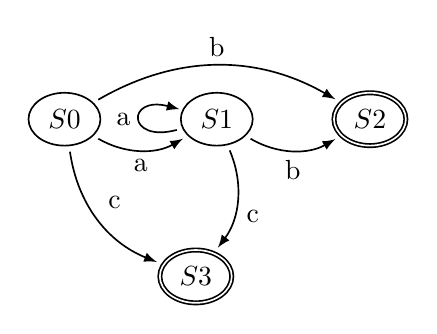
\begin{tikzpicture}[node distance=\dy and \dx,
        >=latex,shorten >=2pt,shorten <=2pt,auto,
        semithick  %semithick, thick, thin semithick
        ]
        \newState{S0}{$S0$}{}{}
        \newState{S1}{$S1$}{right=of S0}{}
       \newState{S2}{$S2$}{right=of S1}{accepting}
         \newState{S3}{$S3$}{below right=of S0}{accepting}
       \newTransition{S0}{S1}{a}{below,bend right}
        \newTransition{S0}{S2}{b}{bend left}
        \newTransition{S1}{S1}{a}{loop left}
        \newTransition{S1}{S2}{b}{below, bend right}
        \newTransition{S1}{S3}{c}{bend left}
        \newTransition{S0}{S3}{c}{bend right}
        \end{tikzpicture}
        \end{center}

\end{frame}

\section{Summary}

\begin{frame}{What you need to know}
\begin{itemize}
\item Regular expressions and FSA are ``equivalent'' (accept/generate the same set of strings (language))
\item Regular expressions can be used to search for patterns
\item Regular languages are the least expressive in the Chomsky hierarchy
\item Models of language differ in their expressive power
\item A formal grammar generates/accepts a language (a set of strings)
\item An FSA accepts all strings from the regular language that it describes
\item FSA operations: Disjunction, Concatenation, Kleene closure
\item Algorithm to convert FSA to RegEx (optionally: and vice versa)
\item Syntax of RegEx and how to use them in python
\end{itemize}
\end{frame}

\end{document}

%%% Local Variables:
%%% mode: latex
%%% TeX-master: t
%%% End:
